\documentclass{standalone}
\usepackage{tikz}
\usetikzlibrary{patterns, positioning}


\begin{document}
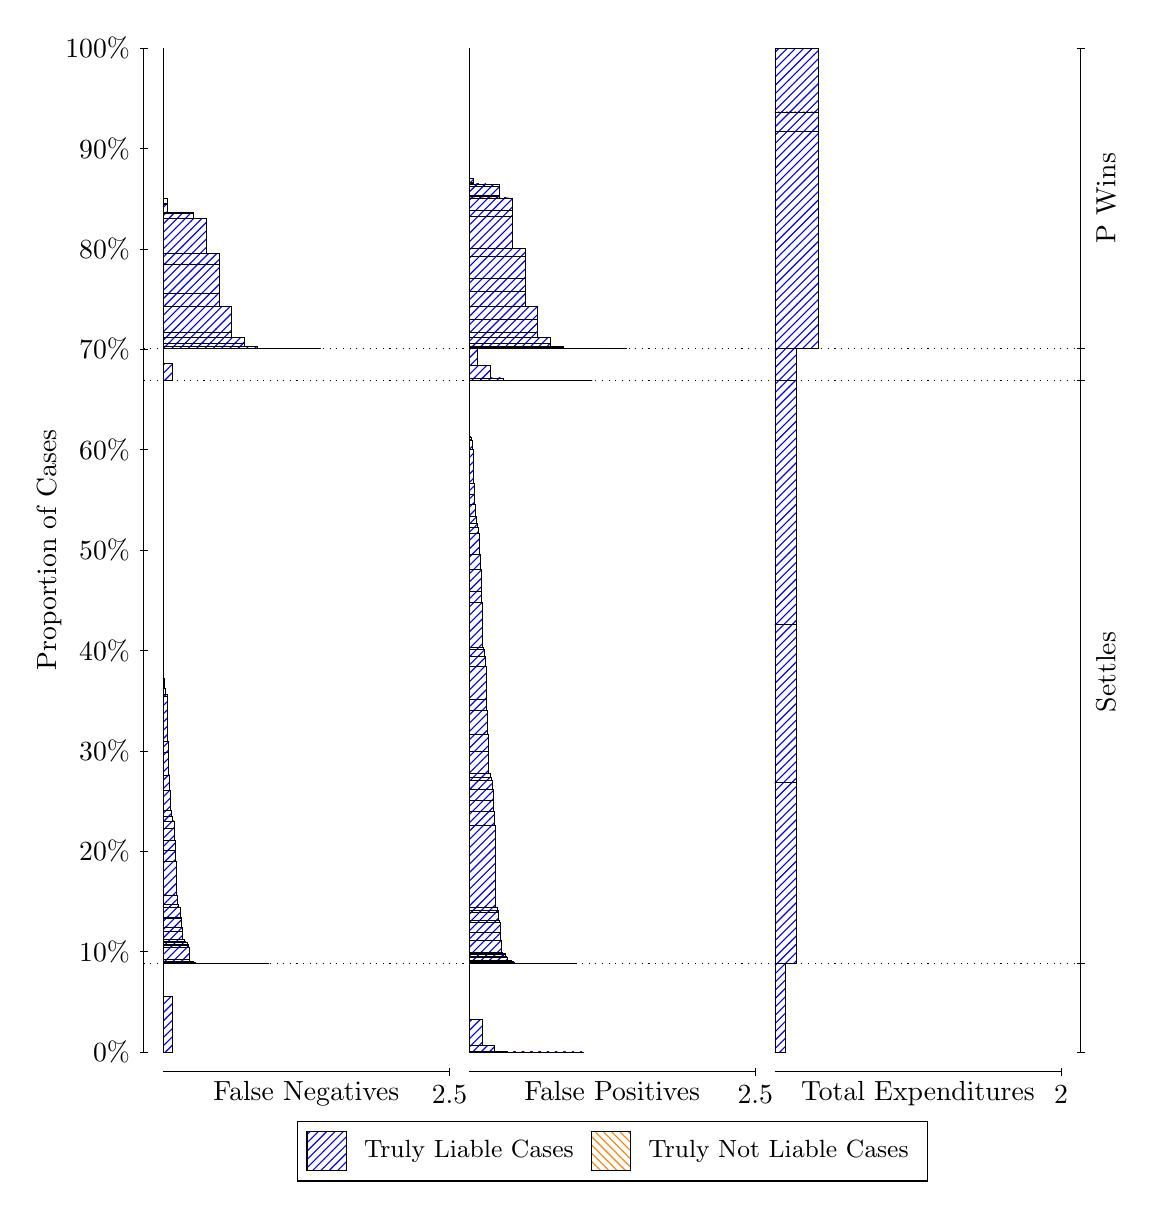
\begin{tikzpicture}
\draw[black, very thin] (1.5,1.75) -- (1.5,14.5);
\node[rotate=90, text=black, anchor=center] at (0.3, 8.125) {Proportion of Cases};
\draw[black, very thin] (1.45,1.75) -- (1.55,1.75);
\node[text=black, anchor=east] at (1.45, 1.75) {0\%};
\draw[black, very thin] (1.45,3.025) -- (1.55,3.025);
\node[text=black, anchor=east] at (1.45, 3.025) {10\%};
\draw[black, very thin] (1.45,4.3) -- (1.55,4.3);
\node[text=black, anchor=east] at (1.45, 4.3) {20\%};
\draw[black, very thin] (1.45,5.575) -- (1.55,5.575);
\node[text=black, anchor=east] at (1.45, 5.575) {30\%};
\draw[black, very thin] (1.45,6.85) -- (1.55,6.85);
\node[text=black, anchor=east] at (1.45, 6.85) {40\%};
\draw[black, very thin] (1.45,8.125) -- (1.55,8.125);
\node[text=black, anchor=east] at (1.45, 8.125) {50\%};
\draw[black, very thin] (1.45,9.4) -- (1.55,9.4);
\node[text=black, anchor=east] at (1.45, 9.4) {60\%};
\draw[black, very thin] (1.45,10.675) -- (1.55,10.675);
\node[text=black, anchor=east] at (1.45, 10.675) {70\%};
\draw[black, very thin] (1.45,11.95) -- (1.55,11.95);
\node[text=black, anchor=east] at (1.45, 11.95) {80\%};
\draw[black, very thin] (1.45,13.225) -- (1.55,13.225);
\node[text=black, anchor=east] at (1.45, 13.225) {90\%};
\draw[black, very thin] (1.45,14.5) -- (1.55,14.5);
\node[text=black, anchor=east] at (1.45, 14.5) {100\%};

\draw[black, very thin] (13.4,1.75) -- (13.4,14.5);
\draw[black, very thin] (13.35,1.75) -- (13.45,1.75);
\node[anchor=west] at (13.35, 1.75) {};
\draw[black, very thin] (13.35,2.8721) -- (13.45,2.8721);
\node[anchor=west] at (13.35, 2.8721) {};
\draw[black, very thin] (13.35,10.276) -- (13.45,10.276);
\node[anchor=west] at (13.35, 10.276) {};
\draw[black, very thin] (13.35,10.684) -- (13.45,10.684);
\node[anchor=west] at (13.35, 10.684) {};
\draw[black, very thin] (13.35,14.5) -- (13.45,14.5);
\node[anchor=west] at (13.35, 14.5) {};

\draw[black, very thin, pattern color=blue, pattern=north east lines] (1.75,1.75) rectangle (1.859,2.4561);
\draw[black, very thin, pattern color=orange, pattern=north west lines] (1.75,2.4561) rectangle (1.75,2.4561);
\draw[black, very thin, pattern color=blue, pattern=north east lines] (1.75,2.4561) rectangle (1.75,2.8721);
\draw[black, very thin, pattern color=blue, pattern=north east lines] (1.75,2.8721) rectangle (3.0943,2.8721);
\draw[black, very thin, pattern color=blue, pattern=north east lines] (1.75,2.8721) rectangle (3.0217,2.8721);
\draw[black, very thin, pattern color=blue, pattern=north east lines] (1.75,2.8721) rectangle (2.949,2.8721);
\draw[black, very thin, pattern color=blue, pattern=north east lines] (1.75,2.8721) rectangle (2.9329,2.8721);
\draw[black, very thin, pattern color=blue, pattern=north east lines] (1.75,2.8721) rectangle (2.8763,2.8721);
\draw[black, very thin, pattern color=blue, pattern=north east lines] (1.75,2.8721) rectangle (2.8602,2.8721);
\draw[black, very thin, pattern color=blue, pattern=north east lines] (1.75,2.8721) rectangle (2.8037,2.8721);
\draw[black, very thin, pattern color=blue, pattern=north east lines] (1.75,2.8721) rectangle (2.7875,2.8721);
\draw[black, very thin, pattern color=blue, pattern=north east lines] (1.75,2.8721) rectangle (2.7714,2.8721);
\draw[black, very thin, pattern color=blue, pattern=north east lines] (1.75,2.8721) rectangle (2.731,2.8721);
\draw[black, very thin, pattern color=blue, pattern=north east lines] (1.75,2.8721) rectangle (2.7149,2.8721);
\draw[black, very thin, pattern color=blue, pattern=north east lines] (1.75,2.8721) rectangle (2.6987,2.8721);
\draw[black, very thin, pattern color=blue, pattern=north east lines] (1.75,2.8721) rectangle (2.6583,2.8721);
\draw[black, very thin, pattern color=blue, pattern=north east lines] (1.75,2.8721) rectangle (2.6422,2.8721);
\draw[black, very thin, pattern color=blue, pattern=north east lines] (1.75,2.8721) rectangle (2.626,2.8721);
\draw[black, very thin, pattern color=blue, pattern=north east lines] (1.75,2.8721) rectangle (2.6099,2.8721);
\draw[black, very thin, pattern color=blue, pattern=north east lines] (1.75,2.8721) rectangle (2.5857,2.8721);
\draw[black, very thin, pattern color=blue, pattern=north east lines] (1.75,2.8721) rectangle (2.5695,2.8721);
\draw[black, very thin, pattern color=blue, pattern=north east lines] (1.75,2.8721) rectangle (2.5534,2.8721);
\draw[black, very thin, pattern color=blue, pattern=north east lines] (1.75,2.8721) rectangle (2.5372,2.8721);
\draw[black, very thin, pattern color=blue, pattern=north east lines] (1.75,2.8721) rectangle (2.513,2.8721);
\draw[black, very thin, pattern color=blue, pattern=north east lines] (1.75,2.8721) rectangle (2.4969,2.8721);
\draw[black, very thin, pattern color=blue, pattern=north east lines] (1.75,2.8721) rectangle (2.4807,2.8721);
\draw[black, very thin, pattern color=blue, pattern=north east lines] (1.75,2.8721) rectangle (2.4646,2.8721);
\draw[black, very thin, pattern color=blue, pattern=north east lines] (1.75,2.8721) rectangle (2.4484,2.8721);
\draw[black, very thin, pattern color=blue, pattern=north east lines] (1.75,2.8721) rectangle (2.4403,2.8721);
\draw[black, very thin, pattern color=blue, pattern=north east lines] (1.75,2.8721) rectangle (2.4242,2.8721);
\draw[black, very thin, pattern color=blue, pattern=north east lines] (1.75,2.8721) rectangle (2.408,2.8721);
\draw[black, very thin, pattern color=blue, pattern=north east lines] (1.75,2.8721) rectangle (2.3919,2.8721);
\draw[black, very thin, pattern color=blue, pattern=north east lines] (1.75,2.8721) rectangle (2.3757,2.8721);
\draw[black, very thin, pattern color=blue, pattern=north east lines] (1.75,2.8721) rectangle (2.3677,2.8721);
\draw[black, very thin, pattern color=blue, pattern=north east lines] (1.75,2.8721) rectangle (2.3515,2.8721);
\draw[black, very thin, pattern color=blue, pattern=north east lines] (1.75,2.8721) rectangle (2.3354,2.8721);
\draw[black, very thin, pattern color=blue, pattern=north east lines] (1.75,2.8721) rectangle (2.3192,2.8722);
\draw[black, very thin, pattern color=blue, pattern=north east lines] (1.75,2.8722) rectangle (2.3031,2.8722);
\draw[black, very thin, pattern color=blue, pattern=north east lines] (1.75,2.8722) rectangle (2.295,2.8722);
\draw[black, very thin, pattern color=blue, pattern=north east lines] (1.75,2.8722) rectangle (2.2869,2.8723);
\draw[black, very thin, pattern color=blue, pattern=north east lines] (1.75,2.8723) rectangle (2.2789,2.8723);
\draw[black, very thin, pattern color=blue, pattern=north east lines] (1.75,2.8723) rectangle (2.2627,2.8723);
\draw[black, very thin, pattern color=blue, pattern=north east lines] (1.75,2.8723) rectangle (2.2466,2.8728);
\draw[black, very thin, pattern color=blue, pattern=north east lines] (1.75,2.8728) rectangle (2.2304,2.8733);
\draw[black, very thin, pattern color=blue, pattern=north east lines] (1.75,2.8733) rectangle (2.2223,2.8736);
\draw[black, very thin, pattern color=blue, pattern=north east lines] (1.75,2.8736) rectangle (2.2143,2.8741);
\draw[black, very thin, pattern color=blue, pattern=north east lines] (1.75,2.8741) rectangle (2.2062,2.8742);
\draw[black, very thin, pattern color=blue, pattern=north east lines] (1.75,2.8742) rectangle (2.19,2.8744);
\draw[black, very thin, pattern color=blue, pattern=north east lines] (1.75,2.8744) rectangle (2.1739,2.8758);
\draw[black, very thin, pattern color=blue, pattern=north east lines] (1.75,2.8758) rectangle (2.1577,2.8823);
\draw[black, very thin, pattern color=blue, pattern=north east lines] (1.75,2.8823) rectangle (2.1497,2.8871);
\draw[black, very thin, pattern color=blue, pattern=north east lines] (1.75,2.8871) rectangle (2.1416,2.8937);
\draw[black, very thin, pattern color=blue, pattern=north east lines] (1.75,2.8937) rectangle (2.1335,2.8943);
\draw[black, very thin, pattern color=blue, pattern=north east lines] (1.75,2.8943) rectangle (2.1254,2.8999);
\draw[black, very thin, pattern color=blue, pattern=north east lines] (1.75,2.8999) rectangle (2.1174,2.9006);
\draw[black, very thin, pattern color=blue, pattern=north east lines] (1.75,2.9006) rectangle (2.1012,2.9026);
\draw[black, very thin, pattern color=blue, pattern=north east lines] (1.75,2.9026) rectangle (2.0851,2.9215);
\draw[black, very thin, pattern color=blue, pattern=north east lines] (1.75,2.9215) rectangle (2.077,3.086);
\draw[black, very thin, pattern color=blue, pattern=north east lines] (1.75,3.086) rectangle (2.0689,3.1075);
\draw[black, very thin, pattern color=blue, pattern=north east lines] (1.75,3.1075) rectangle (2.0609,3.1185);
\draw[black, very thin, pattern color=blue, pattern=north east lines] (1.75,3.1185) rectangle (2.0528,3.139);
\draw[black, very thin, pattern color=blue, pattern=north east lines] (1.75,3.139) rectangle (2.0447,3.1455);
\draw[black, very thin, pattern color=blue, pattern=north east lines] (1.75,3.1455) rectangle (2.0286,3.154);
\draw[black, very thin, pattern color=blue, pattern=north east lines] (1.75,3.154) rectangle (2.0124,3.1792);
\draw[black, very thin, pattern color=blue, pattern=north east lines] (1.75,3.1792) rectangle (1.9963,3.2826);
\draw[black, very thin, pattern color=blue, pattern=north east lines] (1.75,3.2826) rectangle (1.9882,3.338);
\draw[black, very thin, pattern color=blue, pattern=north east lines] (1.75,3.338) rectangle (1.9801,3.4447);
\draw[black, very thin, pattern color=blue, pattern=north east lines] (1.75,3.4447) rectangle (1.972,3.4649);
\draw[black, very thin, pattern color=blue, pattern=north east lines] (1.75,3.4649) rectangle (1.964,3.5829);
\draw[black, very thin, pattern color=blue, pattern=north east lines] (1.75,3.5829) rectangle (1.9559,3.594);
\draw[black, very thin, pattern color=blue, pattern=north east lines] (1.75,3.594) rectangle (1.9397,3.6254);
\draw[black, very thin, pattern color=blue, pattern=north east lines] (1.75,3.6254) rectangle (1.9236,3.7463);
\draw[black, very thin, pattern color=blue, pattern=north east lines] (1.75,3.7463) rectangle (1.9155,4.1752);
\draw[black, very thin, pattern color=blue, pattern=north east lines] (1.75,4.1752) rectangle (1.9074,4.3127);
\draw[black, very thin, pattern color=blue, pattern=north east lines] (1.75,4.3127) rectangle (1.8994,4.4404);
\draw[black, very thin, pattern color=blue, pattern=north east lines] (1.75,4.4404) rectangle (1.8913,4.5899);
\draw[black, very thin, pattern color=blue, pattern=north east lines] (1.75,4.5899) rectangle (1.8832,4.6845);
\draw[black, very thin, pattern color=blue, pattern=north east lines] (1.75,4.6845) rectangle (1.8671,4.7387);
\draw[black, very thin, pattern color=blue, pattern=north east lines] (1.75,4.7387) rectangle (1.8509,4.8138);
\draw[black, very thin, pattern color=blue, pattern=north east lines] (1.75,4.8138) rectangle (1.8348,5.0745);
\draw[black, very thin, pattern color=blue, pattern=north east lines] (1.75,5.0745) rectangle (1.8267,5.2694);
\draw[black, very thin, pattern color=blue, pattern=north east lines] (1.75,5.2694) rectangle (1.8186,5.5519);
\draw[black, very thin, pattern color=blue, pattern=north east lines] (1.75,5.5519) rectangle (1.8106,5.6908);
\draw[black, very thin, pattern color=blue, pattern=north east lines] (1.75,5.6908) rectangle (1.8025,6.2621);
\draw[black, very thin, pattern color=blue, pattern=north east lines] (1.75,6.2621) rectangle (1.7944,6.2893);
\draw[black, very thin, pattern color=blue, pattern=north east lines] (1.75,6.2893) rectangle (1.7783,6.3686);
\draw[black, very thin, pattern color=blue, pattern=north east lines] (1.75,6.3686) rectangle (1.7621,6.4941);
\draw[black, very thin, pattern color=blue, pattern=north east lines] (1.75,6.4941) rectangle (1.754,6.9186);
\draw[black, very thin, pattern color=orange, pattern=north west lines] (1.75,6.9186) rectangle (1.75,6.9186);
\draw[black, very thin, pattern color=blue, pattern=north east lines] (1.75,6.9186) rectangle (1.75,10.276);
\draw[black, very thin, pattern color=blue, pattern=north east lines] (1.75,10.276) rectangle (1.859,10.492);
\draw[black, very thin, pattern color=orange, pattern=north west lines] (1.75,10.492) rectangle (1.75,10.492);
\draw[black, very thin, pattern color=blue, pattern=north east lines] (1.75,10.492) rectangle (1.75,10.684);
\draw[black, very thin, pattern color=blue, pattern=north east lines] (1.75,10.684) rectangle (3.7483,10.684);
\draw[black, very thin, pattern color=blue, pattern=north east lines] (1.75,10.684) rectangle (3.5869,10.684);
\draw[black, very thin, pattern color=blue, pattern=north east lines] (1.75,10.684) rectangle (3.4254,10.684);
\draw[black, very thin, pattern color=blue, pattern=north east lines] (1.75,10.684) rectangle (3.2639,10.684);
\draw[black, very thin, pattern color=blue, pattern=north east lines] (1.75,10.684) rectangle (3.2639,10.684);
\draw[black, very thin, pattern color=blue, pattern=north east lines] (1.75,10.684) rectangle (3.1024,10.687);
\draw[black, very thin, pattern color=blue, pattern=north east lines] (1.75,10.687) rectangle (2.9409,10.709);
\draw[black, very thin, pattern color=blue, pattern=north east lines] (1.75,10.709) rectangle (2.7794,10.755);
\draw[black, very thin, pattern color=blue, pattern=north east lines] (1.75,10.755) rectangle (2.7794,10.828);
\draw[black, very thin, pattern color=blue, pattern=north east lines] (1.75,10.828) rectangle (2.7714,10.828);
\draw[black, very thin, pattern color=blue, pattern=north east lines] (1.75,10.828) rectangle (2.618,10.885);
\draw[black, very thin, pattern color=blue, pattern=north east lines] (1.75,10.885) rectangle (2.618,11.222);
\draw[black, very thin, pattern color=blue, pattern=north east lines] (1.75,11.222) rectangle (2.6099,11.222);
\draw[black, very thin, pattern color=blue, pattern=north east lines] (1.75,11.222) rectangle (2.4565,11.383);
\draw[black, very thin, pattern color=blue, pattern=north east lines] (1.75,11.383) rectangle (2.4565,11.76);
\draw[black, very thin, pattern color=blue, pattern=north east lines] (1.75,11.76) rectangle (2.4565,11.892);
\draw[black, very thin, pattern color=blue, pattern=north east lines] (1.75,11.892) rectangle (2.4484,11.892);
\draw[black, very thin, pattern color=blue, pattern=north east lines] (1.75,11.892) rectangle (2.4484,11.892);
\draw[black, very thin, pattern color=blue, pattern=north east lines] (1.75,11.892) rectangle (2.295,12.334);
\draw[black, very thin, pattern color=blue, pattern=north east lines] (1.75,12.334) rectangle (2.2869,12.334);
\draw[black, very thin, pattern color=blue, pattern=north east lines] (1.75,12.334) rectangle (2.1335,12.338);
\draw[black, very thin, pattern color=blue, pattern=north east lines] (1.75,12.338) rectangle (2.1335,12.403);
\draw[black, very thin, pattern color=blue, pattern=north east lines] (1.75,12.403) rectangle (2.1335,12.41);
\draw[black, very thin, pattern color=blue, pattern=north east lines] (1.75,12.41) rectangle (2.1254,12.41);
\draw[black, very thin, pattern color=blue, pattern=north east lines] (1.75,12.41) rectangle (2.1254,12.41);
\draw[black, very thin, pattern color=blue, pattern=north east lines] (1.75,12.41) rectangle (1.972,12.411);
\draw[black, very thin, pattern color=blue, pattern=north east lines] (1.75,12.411) rectangle (1.972,12.411);
\draw[black, very thin, pattern color=blue, pattern=north east lines] (1.75,12.411) rectangle (1.964,12.417);
\draw[black, very thin, pattern color=blue, pattern=north east lines] (1.75,12.417) rectangle (1.8106,12.417);
\draw[black, very thin, pattern color=blue, pattern=north east lines] (1.75,12.417) rectangle (1.8106,12.417);
\draw[black, very thin, pattern color=blue, pattern=north east lines] (1.75,12.417) rectangle (1.8025,12.513);
\draw[black, very thin, pattern color=blue, pattern=north east lines] (1.75,12.513) rectangle (1.8025,12.53);
\draw[black, very thin, pattern color=blue, pattern=north east lines] (1.75,12.53) rectangle (1.8025,12.586);
\draw[black, very thin, pattern color=orange, pattern=north west lines] (1.75,12.586) rectangle (1.75,12.586);
\draw[black, very thin, pattern color=blue, pattern=north east lines] (1.75,12.586) rectangle (1.75,14.5);
\draw[black, very thin, pattern color=orange, pattern=north west lines] (5.6333,1.75) rectangle (7.0867,1.75);
\draw[black, very thin, pattern color=blue, pattern=north east lines] (5.6333,1.75) rectangle (7.0867,1.75);
\draw[black, very thin, pattern color=blue, pattern=north east lines] (5.6333,1.75) rectangle (6.9252,1.75);
\draw[black, very thin, pattern color=blue, pattern=north east lines] (5.6333,1.75) rectangle (6.7637,1.75);
\draw[black, very thin, pattern color=blue, pattern=north east lines] (5.6333,1.75) rectangle (6.6022,1.75);
\draw[black, very thin, pattern color=blue, pattern=north east lines] (5.6333,1.75) rectangle (6.4407,1.75);
\draw[black, very thin, pattern color=blue, pattern=north east lines] (5.6333,1.75) rectangle (6.2793,1.7503);
\draw[black, very thin, pattern color=blue, pattern=north east lines] (5.6333,1.7503) rectangle (6.1178,1.7579);
\draw[black, very thin, pattern color=blue, pattern=north east lines] (5.6333,1.7579) rectangle (5.9563,1.8357);
\draw[black, very thin, pattern color=blue, pattern=north east lines] (5.6333,1.8357) rectangle (5.7948,2.166);
\draw[black, very thin, pattern color=blue, pattern=north east lines] (5.6333,2.166) rectangle (5.6333,2.8721);
\draw[black, very thin, pattern color=orange, pattern=north west lines] (5.6333,2.8721) rectangle (6.9777,2.8721);
\draw[black, very thin, pattern color=blue, pattern=north east lines] (5.6333,2.8721) rectangle (6.9777,2.8721);
\draw[black, very thin, pattern color=orange, pattern=north west lines] (5.6333,2.8721) rectangle (6.905,2.8721);
\draw[black, very thin, pattern color=blue, pattern=north east lines] (5.6333,2.8721) rectangle (6.905,2.8721);
\draw[black, very thin, pattern color=orange, pattern=north west lines] (5.6333,2.8721) rectangle (6.8323,2.8721);
\draw[black, very thin, pattern color=blue, pattern=north east lines] (5.6333,2.8721) rectangle (6.8323,2.8721);
\draw[black, very thin, pattern color=blue, pattern=north east lines] (5.6333,2.8721) rectangle (6.8162,2.8721);
\draw[black, very thin, pattern color=orange, pattern=north west lines] (5.6333,2.8721) rectangle (6.7597,2.8721);
\draw[black, very thin, pattern color=blue, pattern=north east lines] (5.6333,2.8721) rectangle (6.7597,2.8721);
\draw[black, very thin, pattern color=blue, pattern=north east lines] (5.6333,2.8721) rectangle (6.7435,2.8721);
\draw[black, very thin, pattern color=orange, pattern=north west lines] (5.6333,2.8721) rectangle (6.687,2.8721);
\draw[black, very thin, pattern color=blue, pattern=north east lines] (5.6333,2.8721) rectangle (6.687,2.8721);
\draw[black, very thin, pattern color=blue, pattern=north east lines] (5.6333,2.8721) rectangle (6.6709,2.8721);
\draw[black, very thin, pattern color=blue, pattern=north east lines] (5.6333,2.8721) rectangle (6.6547,2.8721);
\draw[black, very thin, pattern color=orange, pattern=north west lines] (5.6333,2.8721) rectangle (6.6143,2.8721);
\draw[black, very thin, pattern color=blue, pattern=north east lines] (5.6333,2.8721) rectangle (6.6143,2.8721);
\draw[black, very thin, pattern color=blue, pattern=north east lines] (5.6333,2.8721) rectangle (6.5982,2.8721);
\draw[black, very thin, pattern color=blue, pattern=north east lines] (5.6333,2.8721) rectangle (6.582,2.8721);
\draw[black, very thin, pattern color=orange, pattern=north west lines] (5.6333,2.8721) rectangle (6.5417,2.8721);
\draw[black, very thin, pattern color=blue, pattern=north east lines] (5.6333,2.8721) rectangle (6.5417,2.8721);
\draw[black, very thin, pattern color=blue, pattern=north east lines] (5.6333,2.8721) rectangle (6.5255,2.8721);
\draw[black, very thin, pattern color=blue, pattern=north east lines] (5.6333,2.8721) rectangle (6.5094,2.8721);
\draw[black, very thin, pattern color=blue, pattern=north east lines] (5.6333,2.8721) rectangle (6.4932,2.8721);
\draw[black, very thin, pattern color=orange, pattern=north west lines] (5.6333,2.8721) rectangle (6.469,2.8721);
\draw[black, very thin, pattern color=blue, pattern=north east lines] (5.6333,2.8721) rectangle (6.469,2.8721);
\draw[black, very thin, pattern color=blue, pattern=north east lines] (5.6333,2.8721) rectangle (6.4529,2.8721);
\draw[black, very thin, pattern color=blue, pattern=north east lines] (5.6333,2.8721) rectangle (6.4367,2.8721);
\draw[black, very thin, pattern color=blue, pattern=north east lines] (5.6333,2.8721) rectangle (6.4206,2.8721);
\draw[black, very thin, pattern color=orange, pattern=north west lines] (5.6333,2.8721) rectangle (6.3963,2.8721);
\draw[black, very thin, pattern color=blue, pattern=north east lines] (5.6333,2.8721) rectangle (6.3963,2.8721);
\draw[black, very thin, pattern color=blue, pattern=north east lines] (5.6333,2.8721) rectangle (6.3802,2.8721);
\draw[black, very thin, pattern color=blue, pattern=north east lines] (5.6333,2.8721) rectangle (6.364,2.8725);
\draw[black, very thin, pattern color=blue, pattern=north east lines] (5.6333,2.8725) rectangle (6.3479,2.8726);
\draw[black, very thin, pattern color=blue, pattern=north east lines] (5.6333,2.8726) rectangle (6.3317,2.8726);
\draw[black, very thin, pattern color=orange, pattern=north west lines] (5.6333,2.8726) rectangle (6.3237,2.8726);
\draw[black, very thin, pattern color=blue, pattern=north east lines] (5.6333,2.8726) rectangle (6.3237,2.8726);
\draw[black, very thin, pattern color=blue, pattern=north east lines] (5.6333,2.8726) rectangle (6.3075,2.8727);
\draw[black, very thin, pattern color=blue, pattern=north east lines] (5.6333,2.8727) rectangle (6.2914,2.8727);
\draw[black, very thin, pattern color=blue, pattern=north east lines] (5.6333,2.8727) rectangle (6.2752,2.8744);
\draw[black, very thin, pattern color=blue, pattern=north east lines] (5.6333,2.8744) rectangle (6.2591,2.8749);
\draw[black, very thin, pattern color=orange, pattern=north west lines] (5.6333,2.8749) rectangle (6.251,2.8749);
\draw[black, very thin, pattern color=blue, pattern=north east lines] (5.6333,2.8749) rectangle (6.251,2.8751);
\draw[black, very thin, pattern color=blue, pattern=north east lines] (5.6333,2.8751) rectangle (6.2349,2.8752);
\draw[black, very thin, pattern color=blue, pattern=north east lines] (5.6333,2.8752) rectangle (6.2187,2.8754);
\draw[black, very thin, pattern color=blue, pattern=north east lines] (5.6333,2.8754) rectangle (6.2026,2.8932);
\draw[black, very thin, pattern color=blue, pattern=north east lines] (5.6333,2.8932) rectangle (6.1864,2.9019);
\draw[black, very thin, pattern color=orange, pattern=north west lines] (5.6333,2.9019) rectangle (6.1783,2.9019);
\draw[black, very thin, pattern color=blue, pattern=north east lines] (5.6333,2.9019) rectangle (6.1783,2.9034);
\draw[black, very thin, pattern color=blue, pattern=north east lines] (5.6333,2.9034) rectangle (6.1703,2.9088);
\draw[black, very thin, pattern color=blue, pattern=north east lines] (5.6333,2.9088) rectangle (6.1622,2.9096);
\draw[black, very thin, pattern color=blue, pattern=north east lines] (5.6333,2.9096) rectangle (6.146,2.9116);
\draw[black, very thin, pattern color=blue, pattern=north east lines] (5.6333,2.9116) rectangle (6.1299,2.9123);
\draw[black, very thin, pattern color=blue, pattern=north east lines] (5.6333,2.9123) rectangle (6.1137,2.9518);
\draw[black, very thin, pattern color=orange, pattern=north west lines] (5.6333,2.9518) rectangle (6.1057,2.9518);
\draw[black, very thin, pattern color=blue, pattern=north east lines] (5.6333,2.9518) rectangle (6.1057,2.9714);
\draw[black, very thin, pattern color=blue, pattern=north east lines] (5.6333,2.9714) rectangle (6.0976,2.9919);
\draw[black, very thin, pattern color=blue, pattern=north east lines] (5.6333,2.9919) rectangle (6.0895,2.9996);
\draw[black, very thin, pattern color=blue, pattern=north east lines] (5.6333,2.9996) rectangle (6.0734,3.0041);
\draw[black, very thin, pattern color=blue, pattern=north east lines] (5.6333,3.0041) rectangle (6.0572,3.0127);
\draw[black, very thin, pattern color=blue, pattern=north east lines] (5.6333,3.0127) rectangle (6.0411,3.1711);
\draw[black, very thin, pattern color=orange, pattern=north west lines] (5.6333,3.1711) rectangle (6.033,3.1711);
\draw[black, very thin, pattern color=blue, pattern=north east lines] (5.6333,3.1711) rectangle (6.033,3.272);
\draw[black, very thin, pattern color=blue, pattern=north east lines] (5.6333,3.272) rectangle (6.0249,3.3934);
\draw[black, very thin, pattern color=blue, pattern=north east lines] (5.6333,3.3934) rectangle (6.0169,3.4208);
\draw[black, very thin, pattern color=blue, pattern=north east lines] (5.6333,3.4208) rectangle (6.0088,3.5279);
\draw[black, very thin, pattern color=blue, pattern=north east lines] (5.6333,3.5279) rectangle (6.0007,3.55);
\draw[black, very thin, pattern color=blue, pattern=north east lines] (5.6333,3.55) rectangle (5.9846,3.5815);
\draw[black, very thin, pattern color=blue, pattern=north east lines] (5.6333,3.5815) rectangle (5.9684,3.5922);
\draw[black, very thin, pattern color=orange, pattern=north west lines] (5.6333,3.5922) rectangle (5.9603,3.5922);
\draw[black, very thin, pattern color=blue, pattern=north east lines] (5.6333,3.5922) rectangle (5.9603,4.6327);
\draw[black, very thin, pattern color=blue, pattern=north east lines] (5.6333,4.6327) rectangle (5.9523,4.8031);
\draw[black, very thin, pattern color=blue, pattern=north east lines] (5.6333,4.8031) rectangle (5.9442,4.9434);
\draw[black, very thin, pattern color=blue, pattern=north east lines] (5.6333,4.9434) rectangle (5.9361,5.0911);
\draw[black, very thin, pattern color=blue, pattern=north east lines] (5.6333,5.0911) rectangle (5.928,5.197);
\draw[black, very thin, pattern color=blue, pattern=north east lines] (5.6333,5.197) rectangle (5.9119,5.2387);
\draw[black, very thin, pattern color=blue, pattern=north east lines] (5.6333,5.2387) rectangle (5.8957,5.2929);
\draw[black, very thin, pattern color=blue, pattern=north east lines] (5.6333,5.2929) rectangle (5.8796,5.569);
\draw[black, very thin, pattern color=blue, pattern=north east lines] (5.6333,5.569) rectangle (5.8715,5.79);
\draw[black, very thin, pattern color=blue, pattern=north east lines] (5.6333,5.79) rectangle (5.8634,6.0868);
\draw[black, very thin, pattern color=blue, pattern=north east lines] (5.6333,6.0868) rectangle (5.8554,6.2296);
\draw[black, very thin, pattern color=blue, pattern=north east lines] (5.6333,6.2296) rectangle (5.8473,6.6541);
\draw[black, very thin, pattern color=blue, pattern=north east lines] (5.6333,6.6541) rectangle (5.8392,6.7796);
\draw[black, very thin, pattern color=blue, pattern=north east lines] (5.6333,6.7796) rectangle (5.8231,6.8588);
\draw[black, very thin, pattern color=blue, pattern=north east lines] (5.6333,6.8588) rectangle (5.8069,6.8861);
\draw[black, very thin, pattern color=blue, pattern=north east lines] (5.6333,6.8861) rectangle (5.7989,7.4574);
\draw[black, very thin, pattern color=blue, pattern=north east lines] (5.6333,7.4574) rectangle (5.7908,7.5962);
\draw[black, very thin, pattern color=blue, pattern=north east lines] (5.6333,7.5962) rectangle (5.7827,7.8787);
\draw[black, very thin, pattern color=blue, pattern=north east lines] (5.6333,7.8787) rectangle (5.7746,8.0737);
\draw[black, very thin, pattern color=blue, pattern=north east lines] (5.6333,8.0737) rectangle (5.7666,8.3344);
\draw[black, very thin, pattern color=blue, pattern=north east lines] (5.6333,8.3344) rectangle (5.7504,8.4095);
\draw[black, very thin, pattern color=blue, pattern=north east lines] (5.6333,8.4095) rectangle (5.7343,8.4637);
\draw[black, very thin, pattern color=blue, pattern=north east lines] (5.6333,8.4637) rectangle (5.7181,8.5583);
\draw[black, very thin, pattern color=blue, pattern=north east lines] (5.6333,8.5583) rectangle (5.71,8.7077);
\draw[black, very thin, pattern color=blue, pattern=north east lines] (5.6333,8.7077) rectangle (5.702,8.8354);
\draw[black, very thin, pattern color=blue, pattern=north east lines] (5.6333,8.8354) rectangle (5.6939,8.973);
\draw[black, very thin, pattern color=blue, pattern=north east lines] (5.6333,8.973) rectangle (5.6858,9.4019);
\draw[black, very thin, pattern color=blue, pattern=north east lines] (5.6333,9.4019) rectangle (5.6777,9.5227);
\draw[black, very thin, pattern color=blue, pattern=north east lines] (5.6333,9.5227) rectangle (5.6616,9.5542);
\draw[black, very thin, pattern color=blue, pattern=north east lines] (5.6333,9.5542) rectangle (5.6454,9.5653);
\draw[black, very thin, pattern color=blue, pattern=north east lines] (5.6333,9.5653) rectangle (5.6374,9.6833);
\draw[black, very thin, pattern color=blue, pattern=north east lines] (5.6333,9.6833) rectangle (5.6333,10.276);
\draw[black, very thin, pattern color=orange, pattern=north west lines] (5.6333,10.276) rectangle (7.1957,10.276);
\draw[black, very thin, pattern color=blue, pattern=north east lines] (5.6333,10.276) rectangle (7.1957,10.276);
\draw[black, very thin, pattern color=blue, pattern=north east lines] (5.6333,10.276) rectangle (7.0342,10.276);
\draw[black, very thin, pattern color=blue, pattern=north east lines] (5.6333,10.276) rectangle (6.8727,10.276);
\draw[black, very thin, pattern color=blue, pattern=north east lines] (5.6333,10.276) rectangle (6.7112,10.276);
\draw[black, very thin, pattern color=blue, pattern=north east lines] (5.6333,10.276) rectangle (6.5497,10.276);
\draw[black, very thin, pattern color=blue, pattern=north east lines] (5.6333,10.276) rectangle (6.3883,10.276);
\draw[black, very thin, pattern color=blue, pattern=north east lines] (5.6333,10.276) rectangle (6.2268,10.278);
\draw[black, very thin, pattern color=blue, pattern=north east lines] (5.6333,10.278) rectangle (6.0653,10.312);
\draw[black, very thin, pattern color=blue, pattern=north east lines] (5.6333,10.312) rectangle (5.9038,10.468);
\draw[black, very thin, pattern color=blue, pattern=north east lines] (5.6333,10.468) rectangle (5.7423,10.684);
\draw[black, very thin, pattern color=orange, pattern=north west lines] (5.6333,10.684) rectangle (7.6317,10.684);
\draw[black, very thin, pattern color=blue, pattern=north east lines] (5.6333,10.684) rectangle (7.6317,10.684);
\draw[black, very thin, pattern color=orange, pattern=north west lines] (5.6333,10.684) rectangle (7.4702,10.684);
\draw[black, very thin, pattern color=blue, pattern=north east lines] (5.6333,10.684) rectangle (7.4702,10.684);
\draw[black, very thin, pattern color=orange, pattern=north west lines] (5.6333,10.684) rectangle (7.3087,10.684);
\draw[black, very thin, pattern color=blue, pattern=north east lines] (5.6333,10.684) rectangle (7.3087,10.684);
\draw[black, very thin, pattern color=blue, pattern=north east lines] (5.6333,10.684) rectangle (7.1472,10.684);
\draw[black, very thin, pattern color=orange, pattern=north west lines] (5.6333,10.684) rectangle (7.1472,10.684);
\draw[black, very thin, pattern color=blue, pattern=north east lines] (5.6333,10.684) rectangle (7.1472,10.684);
\draw[black, very thin, pattern color=orange, pattern=north west lines] (5.6333,10.684) rectangle (6.9857,10.684);
\draw[black, very thin, pattern color=blue, pattern=north east lines] (5.6333,10.684) rectangle (6.9857,10.686);
\draw[black, very thin, pattern color=blue, pattern=north east lines] (5.6333,10.686) rectangle (6.9857,10.687);
\draw[black, very thin, pattern color=blue, pattern=north east lines] (5.6333,10.687) rectangle (6.9857,10.687);
\draw[black, very thin, pattern color=orange, pattern=north west lines] (5.6333,10.687) rectangle (6.8243,10.687);
\draw[black, very thin, pattern color=blue, pattern=north east lines] (5.6333,10.687) rectangle (6.8243,10.705);
\draw[black, very thin, pattern color=blue, pattern=north east lines] (5.6333,10.705) rectangle (6.8243,10.709);
\draw[black, very thin, pattern color=blue, pattern=north east lines] (5.6333,10.709) rectangle (6.6628,10.745);
\draw[black, very thin, pattern color=orange, pattern=north west lines] (5.6333,10.745) rectangle (6.6628,10.745);
\draw[black, very thin, pattern color=blue, pattern=north east lines] (5.6333,10.745) rectangle (6.6628,10.827);
\draw[black, very thin, pattern color=orange, pattern=north west lines] (5.6333,10.827) rectangle (6.6547,10.827);
\draw[black, very thin, pattern color=blue, pattern=north east lines] (5.6333,10.827) rectangle (6.6547,10.827);
\draw[black, very thin, pattern color=blue, pattern=north east lines] (5.6333,10.827) rectangle (6.5013,10.885);
\draw[black, very thin, pattern color=orange, pattern=north west lines] (5.6333,10.885) rectangle (6.5013,10.885);
\draw[black, very thin, pattern color=blue, pattern=north east lines] (5.6333,10.885) rectangle (6.5013,11.053);
\draw[black, very thin, pattern color=blue, pattern=north east lines] (5.6333,11.053) rectangle (6.5013,11.216);
\draw[black, very thin, pattern color=blue, pattern=north east lines] (5.6333,11.216) rectangle (6.4932,11.216);
\draw[black, very thin, pattern color=orange, pattern=north west lines] (5.6333,11.216) rectangle (6.4932,11.216);
\draw[black, very thin, pattern color=blue, pattern=north east lines] (5.6333,11.216) rectangle (6.4932,11.216);
\draw[black, very thin, pattern color=blue, pattern=north east lines] (5.6333,11.216) rectangle (6.3398,11.411);
\draw[black, very thin, pattern color=blue, pattern=north east lines] (5.6333,11.411) rectangle (6.3398,11.576);
\draw[black, very thin, pattern color=blue, pattern=north east lines] (5.6333,11.576) rectangle (6.3398,11.85);
\draw[black, very thin, pattern color=blue, pattern=north east lines] (5.6333,11.85) rectangle (6.3398,11.955);
\draw[black, very thin, pattern color=orange, pattern=north west lines] (5.6333,11.955) rectangle (6.3317,11.955);
\draw[black, very thin, pattern color=blue, pattern=north east lines] (5.6333,11.955) rectangle (6.3317,11.955);
\draw[black, very thin, pattern color=blue, pattern=north east lines] (5.6333,11.955) rectangle (6.3317,11.955);
\draw[black, very thin, pattern color=blue, pattern=north east lines] (5.6333,11.955) rectangle (6.1783,12.362);
\draw[black, very thin, pattern color=blue, pattern=north east lines] (5.6333,12.362) rectangle (6.1783,12.439);
\draw[black, very thin, pattern color=blue, pattern=north east lines] (5.6333,12.439) rectangle (6.1783,12.598);
\draw[black, very thin, pattern color=blue, pattern=north east lines] (5.6333,12.598) rectangle (6.1703,12.598);
\draw[black, very thin, pattern color=orange, pattern=north west lines] (5.6333,12.598) rectangle (6.1703,12.598);
\draw[black, very thin, pattern color=blue, pattern=north east lines] (5.6333,12.598) rectangle (6.1703,12.598);
\draw[black, very thin, pattern color=blue, pattern=north east lines] (5.6333,12.598) rectangle (6.0169,12.616);
\draw[black, very thin, pattern color=blue, pattern=north east lines] (5.6333,12.616) rectangle (6.0169,12.633);
\draw[black, very thin, pattern color=blue, pattern=north east lines] (5.6333,12.633) rectangle (6.0169,12.749);
\draw[black, very thin, pattern color=blue, pattern=north east lines] (5.6333,12.749) rectangle (6.0169,12.767);
\draw[black, very thin, pattern color=blue, pattern=north east lines] (5.6333,12.767) rectangle (6.0088,12.767);
\draw[black, very thin, pattern color=blue, pattern=north east lines] (5.6333,12.767) rectangle (6.0088,12.767);
\draw[black, very thin, pattern color=orange, pattern=north west lines] (5.6333,12.767) rectangle (6.0088,12.767);
\draw[black, very thin, pattern color=blue, pattern=north east lines] (5.6333,12.767) rectangle (6.0088,12.767);
\draw[black, very thin, pattern color=blue, pattern=north east lines] (5.6333,12.767) rectangle (5.8554,12.769);
\draw[black, very thin, pattern color=blue, pattern=north east lines] (5.6333,12.769) rectangle (5.8554,12.773);
\draw[black, very thin, pattern color=blue, pattern=north east lines] (5.6333,12.773) rectangle (5.8473,12.773);
\draw[black, very thin, pattern color=blue, pattern=north east lines] (5.6333,12.773) rectangle (5.8473,12.774);
\draw[black, very thin, pattern color=orange, pattern=north west lines] (5.6333,12.774) rectangle (5.8473,12.774);
\draw[black, very thin, pattern color=blue, pattern=north east lines] (5.6333,12.774) rectangle (5.8473,12.774);
\draw[black, very thin, pattern color=blue, pattern=north east lines] (5.6333,12.774) rectangle (5.8473,12.774);
\draw[black, very thin, pattern color=blue, pattern=north east lines] (5.6333,12.774) rectangle (5.6939,12.774);
\draw[black, very thin, pattern color=blue, pattern=north east lines] (5.6333,12.774) rectangle (5.6939,12.774);
\draw[black, very thin, pattern color=blue, pattern=north east lines] (5.6333,12.774) rectangle (5.6939,12.774);
\draw[black, very thin, pattern color=blue, pattern=north east lines] (5.6333,12.774) rectangle (5.6858,12.781);
\draw[black, very thin, pattern color=blue, pattern=north east lines] (5.6333,12.781) rectangle (5.6858,12.797);
\draw[black, very thin, pattern color=orange, pattern=north west lines] (5.6333,12.797) rectangle (5.6858,12.797);
\draw[black, very thin, pattern color=blue, pattern=north east lines] (5.6333,12.797) rectangle (5.6858,12.84);
\draw[black, very thin, pattern color=blue, pattern=north east lines] (5.6333,12.84) rectangle (5.6858,12.85);
\draw[black, very thin, pattern color=orange, pattern=north west lines] (5.6333,12.85) rectangle (5.6333,12.85);
\draw[black, very thin, pattern color=blue, pattern=north east lines] (5.6333,12.85) rectangle (5.6333,14.5);
\draw[black, very thin, pattern color=orange, pattern=north west lines] (9.5167,1.75) rectangle (9.6529,1.75);
\draw[black, very thin, pattern color=blue, pattern=north east lines] (9.5167,1.75) rectangle (9.6529,2.8721);
\draw[black, very thin, pattern color=orange, pattern=north west lines] (9.5167,2.8721) rectangle (9.7892,2.8721);
\draw[black, very thin, pattern color=blue, pattern=north east lines] (9.5167,2.8721) rectangle (9.7892,5.1726);
\draw[black, very thin, pattern color=orange, pattern=north west lines] (9.5167,5.1726) rectangle (9.7892,5.1726);
\draw[black, very thin, pattern color=blue, pattern=north east lines] (9.5167,5.1726) rectangle (9.7892,7.1802);
\draw[black, very thin, pattern color=orange, pattern=north west lines] (9.5167,7.1802) rectangle (9.7892,7.1802);
\draw[black, very thin, pattern color=blue, pattern=north east lines] (9.5167,7.1802) rectangle (9.7892,10.276);
\draw[black, very thin, pattern color=orange, pattern=north west lines] (9.5167,10.276) rectangle (9.7892,10.276);
\draw[black, very thin, pattern color=blue, pattern=north east lines] (9.5167,10.276) rectangle (9.7892,10.684);
\draw[black, very thin, pattern color=orange, pattern=north west lines] (9.5167,10.684) rectangle (10.062,10.684);
\draw[black, very thin, pattern color=blue, pattern=north east lines] (9.5167,10.684) rectangle (10.062,13.437);
\draw[black, very thin, pattern color=orange, pattern=north west lines] (9.5167,13.437) rectangle (10.062,13.437);
\draw[black, very thin, pattern color=blue, pattern=north east lines] (9.5167,13.437) rectangle (10.062,13.688);
\draw[black, very thin, pattern color=orange, pattern=north west lines] (9.5167,13.688) rectangle (10.062,13.688);
\draw[black, very thin, pattern color=blue, pattern=north east lines] (9.5167,13.688) rectangle (10.062,14.5);
\draw[black, dotted] (1.5,2.8721) -- (13.4,2.8721);
\draw[black, dotted] (1.5,10.276) -- (13.4,10.276);
\draw[black, dotted] (1.5,10.684) -- (13.4,10.684);
\draw[black, very thin] (1.75,1.5) -- (5.3833,1.5);
\node[text=black, anchor=north] at (3.5667, 1.5) {False Negatives};
\draw[black, very thin] (5.3833,1.45) -- (5.3833,1.55);
\node[text=black, anchor=north] at (5.3833, 1.45) {2.5};

\draw[black, very thin] (5.6333,1.5) -- (9.2667,1.5);
\node[text=black, anchor=north] at (7.45, 1.5) {False Positives};
\draw[black, very thin] (9.2667,1.45) -- (9.2667,1.55);
\node[text=black, anchor=north] at (9.2667, 1.45) {2.5};

\draw[black, very thin] (9.5167,1.5) -- (13.15,1.5);
\node[text=black, anchor=north] at (11.333, 1.5) {Total Expenditures};
\draw[black, very thin] (13.15,1.45) -- (13.15,1.55);
\node[text=black, anchor=north] at (13.15, 1.45) {2};


\node[text=black, centered, rotate=90] at (13.72, 6.5741) {Settles};

\node[text=black, centered, rotate=90] at (13.72, 12.592) {P Wins};

\draw (7.449999999999999,1.5) node[draw=none] (baseCoordinate) {};
\begin{scope}[align=center]
        \matrix[scale=0.5, draw=black, below=0.5cm of baseCoordinate, nodes={draw}, column sep=0.1cm]{
            \node[rectangle, draw, minimum width=0.5cm, minimum height=0.5cm, pattern color=blue, pattern=north east lines] {}; &
            \node[draw=none, font=\small, text=black] (B) {Truly Liable Cases}; &
            \node[rectangle, draw, minimum width=0.5cm, minimum height=0.5cm, pattern color=orange, pattern=north west lines] {}; &
            \node[draw=none, font=\small, text=black] (B) {Truly Not Liable Cases}; \\
            };
\end{scope}

\end{tikzpicture}
\end{document}